\documentclass[a4paper,12pt]{article}
\usepackage{amsfonts,amsmath,amssymb,anysize}
\usepackage{bibentry,blindtext,braket,cancel}
\usepackage{fancyhdr,graphicx}
\usepackage{listings,multicol,mathtools}
\usepackage{pdfpages,siunitx,verbatim}
\usepackage{xfrac,xcolor}
\usepackage{wrapfig}

\marginsize{1.4cm}{1.5cm}{1cm}{1cm}
\linespread{1.5}
\setlength{\headheight}{14.49998pt}

\pagestyle{fancy}
\fancyhf{}
\lhead{Phys. 410 Quantum Mechanics and Its Applications I (Term 221)}
\rhead{Formulas Sheet}

\begin{document}
\begin{center}\textbf{\underline{\huge{Formulas Sheet}}}\end{center}

\subsection*{\underline{Physical Constants:}}
\begin{tabular}{lll}
    \hline Quantity                & Symbol, equation                         & Value                                                                          \\
    \hline Speed of light          & $c$                                      & $2.9979 \times 10^{8} \mathrm{~m} \mathrm{~s}^{-1}$                            \\
    Electron charge                & $e$                                      & $1.602 \times 10^{-19} \mathrm{C}$                                             \\
    Planck constant                & $h$                                      & $6.626 \times 10^{-34} \mathrm{Js}$                                            \\
    Planck constant, reduced       & $\hbar=h / 2 \pi$                        & $1.055 \times 10^{-34} \mathrm{~J} \mathrm{~s}$                                \\
    Conversion constant            & $\hbar c$                                & $197.327 \mathrm{MeVfm}=197.327 \mathrm{eVnm}$                                 \\
    \hline Electron mass           & $m_{e}$                                  & $9.109 \times 10^{-31} \mathrm{~kg}=0.511 \mathrm{MeV} / \mathrm{c}^{2}$       \\
    Proton mass                    & $m_{p}$                                  & $1.673 \times 10^{-27} \mathrm{~kg}^{2}=938.272 \mathrm{MeV} / \mathrm{c}^{2}$ \\
    Neutron mass                   & $m_{n}$                                  & $1.675 \times 10^{-27} \mathrm{~kg}=939.566 \mathrm{MeV} / \mathrm{c}^{2}$     \\
    \hline Fine structure constant & $\alpha=e^{2} / \hbar c$                 & $1 / 137.036$                                                                  \\
    Classical electron radius      & $r_{e}=e^{2} / m_{e} c^{2}$              & $2.818 \times 10^{-15} \mathrm{~m}$                                            \\
    Electron Compton wavelength    & $\lambda=h / m_{e} c=r_{e} / \alpha$     & $2.426 \times 10^{-12} \mathrm{~m}$                                            \\
    Proton Compton wavelength      & $\lambda=h / m_{p} c$                    & $1.321 \times 10^{-15} \mathrm{~m}$                                            \\
    Bohr radius                    & $a_{0}=r_{e} / \alpha^{2}$               & $0.529 \times 10^{-10} \mathrm{~m}$                                            \\
    Rydberg energy                 & $\mathcal{R}=m_{e} c^{2} \alpha^{2} / 2$ & $13.606 \mathrm{eV}^{-11} \mathrm{MeV} \mathrm{T}^{-1}$                        \\
    Bohr magneton                  & $\mu_{B}=e \hbar / 2 m_{e}$              & $5.788 \times 10^{-11}$                                                        \\
    Nuclear magneton               & $\mu_{N}=e \hbar / 2 m_{p}$              & $3.152 \times 10^{-14} \mathrm{MeV} \mathrm{T}^{-1}$                           \\
    \hline Avogadro number         & $N_{A}$                                  & $6.022 \times 10^{23} \mathrm{~mol}^{-1}$                                      \\
    Boltzmann constant             & $k$                                      & $1.381 \times 10^{-23} \mathrm{~J} \mathrm{~K}^{-1}$                           \\
                                   &                                          & $=8.617 \times 10^{-5} \mathrm{eV} \mathrm{K}^{-1}$                            \\
    Gas constant                   & $R=N_{A} k$                              & $8.31 \mathrm{~J} \mathrm{~mol}{ }^{-1} \mathrm{~K}^{-1}$                      \\
    Gravitational constant         & $G$                                      & $6.673 \times 10^{-11} \mathrm{~m}^{3} \mathrm{~kg}^{-1} \mathrm{~s}^{-2}$     \\
    Permittivity of free space     & $\epsilon_{0}=1 / \mu_{0} c^{2}$         & $8.854 \times 10^{-12} \mathrm{Fm}^{-1}$                                       \\
    Permeability of free space     & $\mu_{0}$                                & $4 \pi \times 10^{-7} \mathrm{~N} \mathrm{~A}^{-2}$                            \\
    \hline                         &                                          & 
\end{tabular}

\subsection*{\underline{Conversion of units:}}
$1 \mathrm{fm}=10^{-15} \mathrm{~m}$, $1 \mathrm{fm}=10^{-15} \mathrm{~m}, \quad 1$ barn $=10^{-28} \mathrm{~m}^{2}=100 \mathrm{fm}^{2}$, 1 atmosphere $=101325 \mathrm{~Pa}, \quad$ Thermal energy at $T=300 \mathrm{~K}: \quad k T=[38.682]^{-1} \mathrm{eV}$ $0^{\circ} \mathrm{C}=273.15 \mathrm{~K}, \quad 1 \mathrm{eV}=1.602 \times 10^{-19} \mathrm{~J}, \quad 1 \mathrm{eV} / \mathrm{c}^{2}=1.783 \times 10^{-36} \mathrm{~kg}$
\subsection*{\underline{Properties of the Solution of 1D Stationary Schrodinger Equation:}}
\begin{enumerate}
    \item For 1D potential, all stationary solutions are non-degenerate.
    \item Stationary square integrable solution exist only for $E > min{(V(x))}$
    \item If V(x) is real, then $\Psi$(x) can be taken to be real.
    \item Eigenvalues of a Hermitian Hamiltonian are all real.
    \item The eigenfunctions of a Hermitian operator form a complete orthogonal basis set, for smooth potentials.
    \item 1D Schrodinger equation Solution is real up to an over all phase.
    \item For a given 1D even potential the stationary states are either even or odd.
    \item The wave function and its first order space derivative are continuous all over space and in particular at the boundaries of a finite potential.
    \item At boundaries with Dirac delta function potential,
          the wave function is still continuos but the first space derivative of the wavefunction is discontinuous. 
    \item Due to square integrability, physical solution should be finite all over space, no blow ups, in particular at infinity.
    \item The number of nodes (zeros) of the eigenfunction increases by one unit between adjacent states as we move from the ground state (zero nodes) to higher excited states.
    \item Bound states exist only for confining potential (classically between turning points of the potential).
\end{enumerate}
\subsection*{\underline{The Origin of Quantum Physics:}}
\begin{align}
     & E=h\omega
     & p=\frac{h}{\lambda}=\hbar k
     &                                      \\
     & \lambda=\frac{h}{p} = \frac{2\pi}{k}
     & \lambda_C = \frac{h}{mc}
\end{align}

\subsection*{\underline{Blackbody Radiation:}}
Plank energy spectral density: \resizebox{.4\hsize}{!}{$\rho(\nu)=\frac{8\pi h \nu^3}{c^3}\left[ \frac{1}{\exp \left(\frac{h\nu}{k_BT} \right)-1} \right]$}
\vspace{0.3cm}
%\hrule

\subsection*{\underline{Photoelectric Effect:}}
$W$ is the work function of irradiated metal. $V_s$ is the stopping potential.
$$K=\frac{1}{2}\ mv^2=h\nu-W=\frac{hc}{\lambda}-W\ ;\quad K=\frac{1}{2}\ mv^2=|e|V_s\leftrightarrow V_s=\frac{K}{|e|}$$
$$\nu\geq\frac{W}{h}=\nu_{\min};\quad \nu=\frac{1}{T}=\frac{c}{\lambda};\quad \nu=\frac{\omega}{2\pi}$$
% \vspace{0.3cm}
%\hrule

\subsection*{\underline{de Broglie Formula:}}
$$\lambda=\frac{h}{p}=\frac{h}{mv}$$
\vspace{0.3cm}
%\hrule

\subsection*{\underline{Bohr Hydrogen-like Atom:}}
\begin{align*}
     & E_n=-\frac{Z^2}{n^2}R                                       & \  & \quad R=13.6\,\si{\electronvolt}          \\
     & r_n=\frac{a_0}{Z}n^2                                        & \  & \quad a_0=0.53\times10^{-10}\,\si{\metre} \\
     & h\nu=E_n-E_m=Z^2R\left( \frac{1}{m^2}-\frac{1}{n^2} \right) & \  & \quad n>m
\end{align*}

\subsection*{\underline{The Wave Function:}}
$\Psi(x,t)$ obeys Schrodinger's equation, and the normalization condition $\int_{-\infty}^\infty |\Psi(x,t)|^2dx=1$:
\begin{equation}
    \braket{x}=\int_{-\infty}^\infty x|\Psi(x,t)|^2dx;
    \braket{p}=\int_{-\infty}^\infty \Psi^*(x,t)\frac{\hbar}{i}\frac{\partial}{\partial x}\Psi(x,t)dx;
    \braket{Q(\hat{x},\hat{p})}=\int_{-\infty}^\infty \Psi^*(x,t)Q\left( x,\frac{h}{i} \frac{\partial}{\partial x} \right)\Psi(x,t)dx
\end{equation}
\begin{flalign}
     & i\hbar \frac{\partial }{\partial t}\Psi(x,t)=H\Psi(x,t);
     &                                                                                        & \Psi(x,t)=\psi(x)e^{-iEt/\hbar};
     &                                                                                        & H\psi(x)=E\psi(x)
     &                                                                                                                                                                                                               \\
     & \rho(x,t)=|\Psi(x,t)|^2;
     &                                                                                        & \frac{\partial}{\partial t}\rho(\textbf{x},t)+\nabla \cdot \textbf{J}(\textbf{x},t)=0;
     &                                                                                        & J(x,t)=\frac{i\hbar}{2m}\left( \Psi\frac{\partial \Psi^*}{\partial x}-\Psi^*\frac{\partial \Psi}{\partial x} \right)
     &                                                                                                                                                                                                               \\
     & \mathbf{J}(\mathbf{x},t)=\frac{h}{2im}\left( \psi^*\nabla\psi-\psi\nabla\psi^* \right)
     &                                                                                        & p=\frac{\hbar}{i}\nabla;
     &                                                                                        & [x_i,p_j] = i\hbar \ \delta_{i,j}
\end{flalign}

% A Hermitian operator $Q$ obey: $\int\psi^*(x)Q\psi(x)\,dx=\int(Q\psi(x))^*\psi(x)\,dx$, and $Q^\dagger = Q$.\\
Hermitian conjugate $A^\dagger$ is defined by: $\int(A\psi(x))^*\psi(x),dx=\int\psi(x)A^\dagger\psi(x),dx$.
$$ H = - \frac{\hbar^2}{2m} \frac{d}{dx^2} + V(x) $$
\subsection*{\underline{Fourier Transform \& Wavepackets}}
\begin{flalign}
     & \Psi(x)=\frac{1}{\sqrt{2\pi}}\int dk\Phi(k)e^{ikx},
     &                                                                                               & \Phi(k)=\frac{1}{\sqrt{2\pi}}\int dx\Psi(x)e^{-ikx}
     &                                                                                               & \int dx|\Psi(x)|^2 = \int dk|\Phi(k)|^2 = 1
     &                                                                                                                                                                                                   \\
     & \Psi(x)=\frac{1}{(2\pi)^\frac{3}{2}}\int d^3k\Phi(\textbf{k})e^{i\textbf{k}\cdot \textbf{x}},
     &                                                                                               & \Phi(k)=\frac{1}{(2\pi)^\frac{3}{2}}\int d^3x\Psi(\textbf{x})e^{-i\textbf{k}\cdot \textbf{x}}
     &                                                                                               & \int d^x|\Psi(\textbf{x})|^2 = \int d^k|\Phi(\textbf{k})|^2 = 1
     &                                                                                                                                                                                                   \\
     & \frac{1}{2\pi} \int_{-\infty}^\infty e^{ikx}dx = \delta(k)
     &                                                                                               & \frac{1}{(2\pi)^3} \int_{-\infty}^\infty e^{i\textbf{k}\cdot \textbf{x}}d^3x = \delta^{(3)}(k)
     &                                                                                               & \Psi(x,t)=\frac{1}{(2\pi)^3}\int\phi(k)e^{i(\mathbf{k}\cdot\mathbf{x}-\omega(\mathbf{k})t)}\,dk^3
\end{flalign}
\begin{equation}
    v_{group} =\frac{d\omega}{dk};\  \Delta k\Delta x \simeq 1
\end{equation}
\subsection*{\underline{Complete Basis Set:}}
Given that $H\psi_n(x)=E_n\psi_n(x);\quad \int\phi^*_n(x)\phi_m(x)dx=\delta_{nm}$, where $\{\phi_n\}$ is a complete set, then:
\begin{gather}
    \psi(x)=\sum_nc_n\phi_n(x);\quad c_n=\int\psi^*_n(x)\psi(x)\,dx\\
    \int\psi^*(x)\psi(x)dx=\sum_n|c_n|^2=1\\
    E=\int\psi^*_n(x)H\psi_m(x)dx=\sum_n|c_n|^2E_n\\
    \Psi(x,0)=\psi(x)=\sum_nc_n\phi_n(x)\implies\Psi(x,t)
    \begin{cases}
        =\sum_nc_ne^{-iE_nt/\hbar}\phi_n(x) \\
        =e^{i\hat H t/\hbar}\Psi(x,0)       \\
    \end{cases}
    \\ c_n=\int\phi_n^*\Psi(x,0)dx
\end{gather}
\subsection*{\underline{Commutator Properties:}}
\begin{equation}
    [A,A]=0;\quad
    [A,B]=-[B,A];\quad
    [A+B,C]=[A,C]+[B,C]\quad
\end{equation}
\begin{equation}
    [AB,C]=[A,C]B+A[B,C];\quad
    [A,BC]=[A,B]C+B[A,C];\quad
\end{equation}
\begin{equation}
    [A,[B,C]]+[B,[C,A]]+[C,[A,B]]=0
\end{equation}
\subsection*{\underline{Uncertainty Principle:}}
\begin{align}
     & (\Delta Q)^2 = \braket{Q^2} - \braket{Q}^2 = \braket{(Q-\braket{Q})^2}
     & \Delta x \Delta p \geq \frac{\hbar}{2}
\end{align}
Where $\Delta Q$ is the uncertainty for the Hermitian Operator Q.
\begin{align}
    (\Delta{Q})^2 (\Delta{R})^2 \ge \frac{1}{2} \left| \langle [Q, R] \rangle \right| ^2
\end{align}
\subsection*{\underline{Operators:}}
For the operator $\hat{A}$, $\hat{A}\psi=a\psi$. $a$ in an eigenvalue and $\psi$ is an eigenfunction of $A$. Then, the following properties hold:
\begin{itemize}
    \item $\hat{A}^n\psi=a^n\psi,\quad \hat{A}^{-1}\psi=a^{-1}\psi,\quad e^{i\hat{A}}\psi=e^{ia}\psi,\quad F(\hat{A})\psi=F(a)\psi$
    \item If $\hat{A}^{\dagger}=A,\ \hat{A}\ket{\phi_n}=a_n\ket{\phi_n} \quad \implies a_n\in \mathbb{R}, \braket{\phi_m|\phi_n}=\delta_{mn}$
    \item If $\{\phi_n\}$ is a complete and orthonormal for a Hermitian operator, then the operator is diagonal in the eigenbasis, $\{\phi_n\}$, with eigenvalues,, $\{a_n\}$, as the diagonal elements. The basis set is unique iff there are no degenerate eigenvalues.
    \item If two Hermitian operators, $\hat{A}$ and $\hat{B}$, commute and have no degenerate eigenvalues. Then each eigenvector of $\hat{A}$ is also an eigenvector of $\hat{B}$. A common orthonormal basis can be made of the joint eigenvectors of $\hat{A}$ and $\hat{B}$.
\end{itemize}
\subsection*{\underline{1D Infinite Square Well:}}
\begin{align}
     & H\psi_n(x)=E_n\psi_n(x)
     & 
     & \int\psi^*_n(x)\psi_n(x)dx=\delta_{n,m}
    \\
     & \phi_n(x)=\sqrt{\frac{2}{a}}\sin\left( \frac{n\pi}{a}x \right); \, n= 1, 2, \dots
     & 
     & \phi_n(x,t)=\phi_n(x)e^{-iE_nt/\hbar}
    \\
     & V(x)=\left\{\begin{matrix}0, 0\leq x\leq a\\\infty, \mathrm{otherwise}\end{matrix}\right.
     & 
     & E_n=\frac{\hbar^2k_n^2}{2m}=\frac{n^2\pi^2\hbar^2}{2ma^2}
    \\
     & \Psi(x,t)=\sum_{n=1}^\infty c_n\phi_n(x)e^{-iE_nt/\hbar}
     & 
     & c_n=\int_0^a\phi_n(x)\Psi(x,0)\,dx
\end{align}
\subsection*{\underline{Particle on a Ring:}}
\begin{align}
     & \psi_\pm(\theta)=\frac{1}{\sqrt{2\pi}}\exp{\left( \pm i\frac{R\theta}{\hbar}\sqrt{2mE} \right)}
    = \frac{1}{\sqrt{2\pi}}e^{\pm ikx}
     & 
     & x=R\theta; L=2\pi R; k=\frac{2\pi n}{L}=\frac{n}{R}
    \\
     & \psi(\theta)=\frac{1}{\sqrt{2\pi}}\exp{\pm in\theta}
     & 
     & E_n=\frac{n^2\hbar^2}{2mR^2},\quad n=0\pm 1,\pm 2,\pm 3,...
\end{align}
\subsection*{\underline{Harmonic Oscillator:}}
\begin{align}
     & V(x)=\frac{1}{2}kx^2=\frac{1}{2}m(\omega x)^2\quad \left( \omega\equiv\sqrt{k/m} \right)
     & 
     & E_n=\hbar\omega\left( n+\frac{1}{2} \right);n=0,1,2,\dots
    \\
     & H=\frac{1}{2m}[p^2+(m\omega x)^2]=\hbar\omega\left( N+\frac{1}{2} \right)
     & 
     & N=a_+a_-\quad (=a^\dagger a)
    \\
     & N\psi_n=n\psi_n; \, a_\pm = \sqrt{\frac{m \omega}{2 \hbar}} (\hat{x} \mp i \frac{\hat{p}}{m \omega})
     & 
     & N(a_+\psi_n)=[N,a_+]\psi_n
    \\
     & [N,a_\pm]=\pm a_\pm; \, [a_-, a_+] = 1
     & 
     & a_\pm\equiv \frac{1}{\sqrt{2\hbar m\omega}}\left( \mp ip+m\omega x \right)
    \\
     & x=\sqrt{\frac{\hbar}{2m\omega}}\,(a_++a_-)
     & 
     & p=i\sqrt{\frac{m\omega\hbar}{2}}\,(a_+ - a_-)
    \\
     & a_+\psi_n=\sqrt{n+1}\psi_{n+1}
     & 
     & a_-\psi_n=\sqrt{n}\psi_{n-1}
    \\
     & \psi_0(x)=\left( \frac{m\omega}{\pi\hbar} \right)^{1/4}\exp\left( -\frac{m\omega}{2\hbar}x^2 \right)
     & 
     & \psi_n=\frac{1}{\sqrt{n!}}(a_+)^n\psi_0
    \\
     & \xi\equiv\sqrt{\frac{m\omega}{\hbar}}x
     & 
     & \mathcal{H}_n(\xi)=(-1)^ne^{\xi^2}\left( \frac{d}{d\xi} \right)^ne^{-\xi^2}
    \\
     & \psi_n(x)=\left( \frac{m\omega}{\pi\hbar} \right)^{1/4}\frac{1}{\sqrt{2^n n!}}\mathcal{H}_n(\xi)e^{-\xi^2/2}
     & 
     & \int_{-\infty}^{+\infty}\mathcal{H}_n\mathcal{H}_me^{-x^2}dx=2^nn!\sqrt{\pi}\delta_{n,m}
\end{align}
\subsection*{\underline{Models of Dirac Delta Distribution $\delta(x)$:}}
\begin{equation}
    \delta(x)=\lim_{\alpha\rightarrow\infty}\frac{\sin(\alpha x)}{\pi x};\ 
    \delta(x)=\lim_{\epsilon\rightarrow0^+}\frac{1}{2\pi}\int_{-\infty}^{\infty}e^{-ikx}e^{-\epsilon |k|}\,dk=\lim_{\epsilon\rightarrow0^+}\frac{\epsilon}{\pi (x^2+\epsilon^2)};\ 
    \delta(x)=\lim_{\epsilon\rightarrow0}\frac{\Theta(x+\epsilon)-\Theta(\epsilon)}{\epsilon}
\end{equation}
where $\Theta(x)$ is Heaviside or step function,
\begin{align}
    \Theta{(x)} = \begin{cases}
        1 , & x > 0 \\
        0 , & x < 0
    \end{cases}
\end{align}

\subsection*{\underline{Bound State of Single $\delta$-Potential:} \fbox{$E < 0$}}
\begin{align}
     & V=-\alpha\delta(x), \ \alpha>0
     & 
     & \psi(x)=\sqrt{\frac{m\alpha}{\hbar^2}}\ e^{-\frac{m\alpha}{\hbar^2}|x|}
     & 
     & E=-\frac{m\alpha^2}{2\hbar^2}
\end{align}

\subsection*{\underline{Scattering State:} \fbox{$E > 0$}}
\begin{align}
     & V(x)=-\alpha\delta(x);\, k = \frac{\sqrt{2mE}}{\hbar}
     & 
     & \psi(x) = \begin{cases}
        Ae^{ikx}+Be^{-ikx}, & x<0 \\
        Fe^{ikx},           & x>0
    \end{cases}
    \\
     & T=\frac{|F|^2}{|A|^2}=\frac{1}{1+\beta^2}
     & 
     & R=\frac{|B|^2}{|A|^2}=\frac{\beta}{1+\beta}\qquad (\beta=m\alpha/\hbar^2k)
\end{align}
\subsection*{\underline{Miscellaneous:}}
\begin{align}
    \int_{-\infty}^\infty e^{-ax^2}\, dx=\sqrt{\frac{\pi}{a}};
     &  & 
    \int_{-\infty}^\infty e^{-(ax^2+bx)}\,dx=e^{b^2/4a}\sqrt{\frac{\pi}{a}};
     &  & 
    \delta_{ij} =
    \begin{cases}
        1, & i=j     \\
        0, & i\neq j
    \end{cases}
\end{align}
\subsection*{\underline{Matrix Algebra:}}
Let A be a 2X2 matrix defined as:
$A = \begin{bmatrix}
        a & b \\
        c & d
    \end{bmatrix}$ then:
\begin{align}
     &  & A^{-1}=\frac{1}{|A|}
    \begin{bmatrix}
        d  & -b \\
        -c & a
    \end{bmatrix};\, |A| = ad-bc
\end{align}
\begin{align}
    \sigma_x = \begin{bmatrix}
        0 & 1 \\
        1 & 0
    \end{bmatrix} \qquad
    \sigma_y = \begin{bmatrix}
        0 & -1 \\
        i & 0
    \end{bmatrix} \qquad
    \sigma_z = \begin{bmatrix}
        1 & 0  \\
        0 & -1
    \end{bmatrix}
\end{align}
\begin{align}
    \{ \sigma_i, \sigma_j \} = 2 \delta_ij \qquad
    [\sigma_i, \sigma_j] = 2i \in ijk \qquad
    \sigma_i \sigma_j = \begin{cases}
        1 ,                   & i=j      \\
        - \sigma_j \sigma_i , & i \neq j
    \end{cases}
\end{align}
\subsection*{\underline{Orbital Angular Momentum:}}
\begin{gather}
    \hat{L}_{x}=\hat{y} \hat{p}_{z}-\hat{z} \hat{p}_{y}, \quad \hat{L}_{y}=\hat{z} \hat{p}_{x}-\hat{x} \hat{p}_{z}, \quad \hat{L}_{z}=\hat{x} \hat{p}_{y}-\hat{y} \hat{p}_{x} \\
    {\left[\hat{L}_{x}, \hat{L}_{y}\right]=i \hbar \hat{L}_{z}, \quad\left[\hat{L}_{y}, \hat{L}_{z}\right]=i \hbar \hat{L}_{x}, \quad\left[\hat{L}_{z}, \hat{L}_{x}\right]=i \hbar \hat{L}_{y} \cdot} \\
    \hat{L}^{2} \equiv \hat{L}_{x} \hat{L}_{x}+\hat{L}_{y} \hat{L}_{y}+\hat{L}_{z} \hat{L}_{z}, \quad\left[\hat{L}^{2}, \hat{L}_{i}\right]=0 \\
    \nabla=\hat{r}\frac{\partial}{\partial r}+\hat{\theta}\frac{1}{r}\frac{\partial}{\partial \theta}+\hat{\phi}\frac{1}{r\sin\theta}\frac{\partial}{\partial \phi}\\
    \nabla^{2}=\frac{1}{r^2} \frac{\partial}{\partial r}\left( r^2\frac{\partial}{\partial r} \right)
    +\frac{1}{r^{2}\sin\theta}\frac{\partial}{\partial \theta}\left( \sin\theta\frac{\partial}{\partial\theta} \right)
    +\frac{1}{r^{2}\sin^2\theta} \left( \frac{\partial^{2}}{\partial \phi^{2}} \right)\\
    \nabla^{2}=\frac{1}{r} \frac{\partial^{2}}{\partial r^{2}} r+\frac{1}{r^{2}}\left(\frac{\partial^{2}}{\partial \theta^{2}}+\cot \theta \frac{\partial}{\partial \theta}+\frac{1}{\sin ^{2} \theta} \frac{\partial^{2}}{\partial \phi^{2}}\right) \\
    \hat{L}^{2}=-\hbar^{2}\left(\frac{\partial^{2}}{\partial \theta^{2}}+\cot \theta \frac{\partial}{\partial \theta}+\frac{1}{\sin ^{2} \theta} \frac{\partial^{2}}{\partial \phi^{2}}\right) \\
    \hat{L}_{z}=\frac{\hbar}{i} \frac{\partial}{\partial \phi} ; \quad \hat{L}_{\pm}=\hbar e^{\pm i \phi}\left(\pm \frac{\partial}{\partial \theta}+i \cot \theta \frac{\partial}{\partial \phi}\right)=\hat{L}_{x}\pm i\hat{L}_{y}
\end{gather}

\subsection*{\underline{General Momentum Operator} \fbox{$\vec{L},\, \vec{S},\, \vec{J}$}}
\begin{flalign}
     & \left[J_x, J_y\right]=i\hbar J_z
     &                                   & \left[J_z, J_x\right]=i\hbar J_y
     &                                   & \left[J_y, J_z\right]=i\hbar J_x
     &                                                                      \\
     & J^2\ket{Jm}=\hbar^2j(j+1)\ket{Jm}
     &                                   & J_z\ket{Jm}=\hbar m\ket{Jm}
     &                                   & J^2=J^2_x + J^2_y + J^2_z
\end{flalign}
\begin{gather}
    J^2 =J_\pm J_\mp + {J_z}^2\mp\hbar J_z
\end{gather}
$\ket{Jm}$ are common eigenstates of the $J^2,J_z$;\\
Thus both $J^2$ and $J_z$ are diagonal matrices for any fixed value of J, the dimension of these matrices is $(2J+1) \times (2J+1)$ since $m=-J,-J+1,\dots,J-1,J,$ (2J+1 Values).\\
$J=\frac{1}{2}\implies 2J+1=2 \implies 2\times2 \text{ matrices}.\\$
$J=1\implies 2J+1=3 \implies 3\times3\text{ matrices}.$
    \begin{flalign}    
         & J_\pm=J_x \pm iJ_y
         &                    & J_\pm\ket{J m}=\sqrt{J(J+1)-m(m\pm1)}\ket{J m\pm1}
    \end{flalign}
    so that $J_\pm$ are off diagonal matrices.\\
    We oreder the eigenvectors for a fixed J-value as the following:\\
$\ket{J,J}\quad\ket{J,J-1}\quad\ket{J,J-2}\quad \dots \quad\ket{J,-J}$\\
    For a fixed J here is the expectation of operator A:
    \begin{equation}
        A = 
        \left(\begin{matrix}
            \bra J A \ket J     & \bra J A \ket {J-1}   & \dots  & \bra J A \ket {-J}     \\
            \bra{ J-1} A \ket J & \bra{J-1} A \ket{J-1} & \dots  & \bra{ J-1} A \ket {-J} \\
            \vdots              & \vdots                & \vdots & \vdots                 \\
            \bra{-J} A \ket J   & \bra{-J} A \ket{J-1}  & \dots  & \bra{- J} A \ket {-J}
        \end{matrix}\right)
    \end{equation}
    in the above matrix, for a fixed J we denote $\ket{J m}=\ket m$.
    
    \subsection*{\underline{Spin Angular Momentum Operator}}
    For $j=\frac{1}{2}\implies \ket{\uparrow} = \ket{\frac{1}{2},\frac{1}{2}}; \ket{\downarrow} = \ket{\frac{1}{2},-\frac{1}{2}} then:$
\begin{flalign}
     & S_x=\frac{\hbar}{2}\left(
    \begin{matrix}
            0 & 1 \\
            1 & 0
        \end{matrix}\right) = \frac{\hbar}{2}\sigma_1
     &                                  & S_y=\frac{\hbar}{2}\left(
    \begin{matrix}
            0 & -i \\
            i & 0
        \end{matrix}\right) = \frac{\hbar}{2}\sigma_2
     &                                  & S_z=\frac{\hbar}{2}\left(
    \begin{matrix}
            1 & 0  \\
            0 & -1
        \end{matrix}\right) = \frac{\hbar}{2}\sigma_3
     &                                                                     \\
     & \left[S_x, S_y\right]=i\hbar S_z
     &                                  & \left[S_z, S_x\right]=i\hbar S_y
     &                                  & \left[S_y, S_z\right]=i\hbar S_x
     &                                                                     \\
     & S_+=S_x+iS_y
     &                                  & S_-=S_x-iS_y
     &                                                                     \\
     & S_+=\frac{\hbar}{2}\left(
    \begin{matrix}
            0 & 2 \\
            0 & 0
        \end{matrix}\right)
     &                                  & S_-=\frac{\hbar}{2}\left(
    \begin{matrix}
            0 & 0 \\
            2 & 0
        \end{matrix}\right)
\end{flalign}
\subsection*{\underline{Spherical Harmonics:}}
\begin{gather}
    \langle \theta\, \phi | l \,m \rangle = Y_{\ell, m}(\theta, \phi) \equiv \mathcal{N}_{\ell, m} P_{\ell}^{m}(\cos \theta) e^{i m \phi}\\
    \hat{L}_{z} Y_{\ell m}=\hbar m Y_{\ell m}\\
    \hat{L}^{2} Y_{\ell m}=\hbar^{2} \ell(\ell+1) Y_{\ell m}\\
    \langle l' \,m' | l \,m \rangle = \int d \Omega Y_{\ell^{\prime} m^{\prime}}^{*}(\theta, \phi) Y_{\ell m}(\theta, \phi)=\delta_{\ell^{\prime}, \ell} \delta_{m^{\prime}, m}, \quad \int d \Omega=\int_{0}^{2 \pi} d \phi \int_{-1}^{1} d(\cos \theta)\\
    Y_{0,0}(\theta, \phi)=\frac{1}{\sqrt{4 \pi}} ; \quad Y_{1, \pm 1}(\theta, \phi)=\mp \sqrt{\frac{3}{8 \pi}} \sin \theta \exp (\pm i \phi) ; \quad Y_{1,0}(\theta, \phi)=\sqrt{\frac{3}{4 \pi}} \cos \theta \\
    \int |\theta \, \phi \rangle \langle \theta \, \phi | \, d\Omega = 1 \qquad \sum_{lm} | l \, m \rangle \langle l \, m | = 1
\end{gather}
\subsection*{\underline{Central Potentials $V(\mathbf{r})=V(r)$:}}
\begin{gather}
    \left[ \frac{-\hbar^2}{2m}\nabla^2+V(r) \right]\psi(r,\theta,\phi)=E\psi(r,\theta,\phi)\\
    -\frac{\hbar^2}{2m}\left[ \frac{1}{r}\frac{\partial^2}{\partial r^2}r- \frac{L^2(\theta,\phi)}{\hbar^2r^2}+V(r)\right]\psi(r,\theta,\phi)=E\psi(r,\theta,\phi)\\
    \psi(r, \theta, \phi)=R(r)Y_{l,m}*(\theta\phi)\\
    \psi(r, \theta, \phi)=\frac{u(r)}{r} Y_{\ell m}(\theta, \phi)\\
    \left(-\frac{\hbar^{2}}{2 m} \frac{d^{2}}{d r^{2}}+V(r)+\frac{\hbar^{2} \ell(\ell+1)}{2 m r^{2}}\right) u(r)=E u(r)\\
    u(r) \sim r^{\ell+1},\ \text{as} \, r \rightarrow 0 \\
    \left[ -\frac{\hbar^2}{2m} \frac{d^2}{dr^2} + V_{\text{eff}}(r) \right] u(r) = E\, u(r); \qquad V_{\text{eff}}(r) = V(r) + \frac{\hbar^2 \ell (\ell +1)}{2m r^2} \\
    \nabla^{2}=\frac{1}{r} \frac{\partial^{2}}{\partial r^{2}} r+\frac{1}{r^{2}}\left(\frac{\partial^{2}}{\partial \theta^{2}}+\cot \theta \frac{\partial}{\partial \theta}+\frac{1}{\sin ^{2} \theta} \frac{\partial^{2}}{\partial \phi^{2}}\right) \\
    \hat{L}^{2}=-\hbar^{2}\left(\frac{\partial^{2}}{\partial \theta^{2}}+\cot \theta \frac{\partial}{\partial \theta}+\frac{1}{\sin ^{2} \theta} \frac{\partial^{2}}{\partial \phi^{2}}\right) \\
    \hat{L}_{z}=\frac{\hbar}{i} \frac{\partial}{\partial \phi} ; \quad \hat{L}_{\pm}=\hbar e^{\pm i \phi}\left(\pm \frac{\partial}{\partial \theta}+i \cot \theta \frac{\partial}{\partial \phi}\right)=\hat{L}_{x}\pm i\hat{L}_{y}
\end{gather}
\subsection*{\underline{Hydrogen Atom (Z=1):}}
\begin{gather}
    V(r) = - \frac{Z e^2}{r} \qquad V_\text{eff}(r) = - \frac{Z e^2}{r} + \frac{\hbar^2 \ell (\ell +1)}{2m r^2} \\
    H=\frac{\mathbf{p}^{2}}{2 m}-\frac{Z e^{2}}{r} \\
    E_{n}=-\frac{Z^{2} e^{2}}{2 a_{0}} \frac{1}{n^{2}}, \quad a_{0}=\frac{\hbar^{2}}{m e^{2}} \simeq 0.529 \times 10^{-10} \mathrm{~m}, \quad \frac{e^{2}}{2 a_{0}} \simeq 13.6 \mathrm{eV} \\
    \psi_{n \ell m}(r, \theta,\phi)=A\left(\frac{r}{a_{0}}\right)^{\ell}\left(\text { Polynomial in } \frac{r}{a_{0}} \text { of degree } n-(\ell+1)\right) e^{-\frac{Z_{r}}{n a_{0}}} {Y_{\ell}^m}(\theta, \phi) \\
    \psi_{n\ell m}(r, \theta, \phi) = R_{n \ell}(r){Y_{\ell}^m}(\theta, \phi)= \sqrt{\left(\frac{2}{na}\right)^3\frac{\left(n-\ell-1\right)!}{2n(n+\ell)!}}e^{\frac{-r}{na}}\left(\frac{2r}{na}\right)^\ell [L_{n-\ell-1}^{2\ell+1}\left(\frac{2r}{na}\right)]{Y_{\ell}^m}(\theta, \phi)\\
    \int\psi^*_{n \ell m}(\vec{r})\psi_{n' \ell ' m'}(\vec{r})d^3\vec r=\delta_{nn'}\delta_{mm'}\delta_{\ell\ell '}\\
    \hat{H}\psi_{n \ell m}(\vec{r}) = E_n\psi_{n \ell m}(\vec{r})\\
    n=1,2, \ldots, \quad \ell=0,1, \ldots, n-1, \quad m=-\ell, \ldots, \ell \\
    \psi_{n\ell m}(r, \theta, \phi)=\frac{u_{n \ell}(r)}{r} {Y_{\ell}^m}(\theta, \phi) \\
    u_{1,0}(r)=\frac{2 r}{a_{0}^{3 / 2}} \exp \left(-r / a_{0}\right) \\
    u_{2,0}(r)=\frac{2 r}{\left(2 a_{0}\right)^{3 / 2}}\left(1-\frac{r}{2 a_{0}}\right) \exp \left(-r / 2 a_{0}\right) \\
    u_{2,1}(r)=\frac{1}{\sqrt{3}} \frac{1}{\left(2 a_{0}\right)^{3 / 2}} \frac{r^{2}}{a_{0}} \exp \left(-r / 2 a_{0}\right) \\
    \Psi_{100}(r, \theta, \phi) = \frac{2r}{\sqrt{4 \pi a_0^3}} e^{-r/a_0}
\end{gather}
\subsection*{\underline{Transfer Matrix}} % (fold)
\label{sub:Transfer Matrix}
\begin{align}
    \begin{bmatrix}
        F \\ G
    \end{bmatrix} = M \begin{bmatrix}
        A \\ B
    \end{bmatrix} \qquad
    M = \begin{bmatrix}
        M_{11}   & M_{12}   \\ 
        M^*_{12} & M^*_{11}
    \end{bmatrix} \qquad
    \det{M} = 1
\end{align}
\begin{wrapfigure}{r}{0.35\linewidth}
    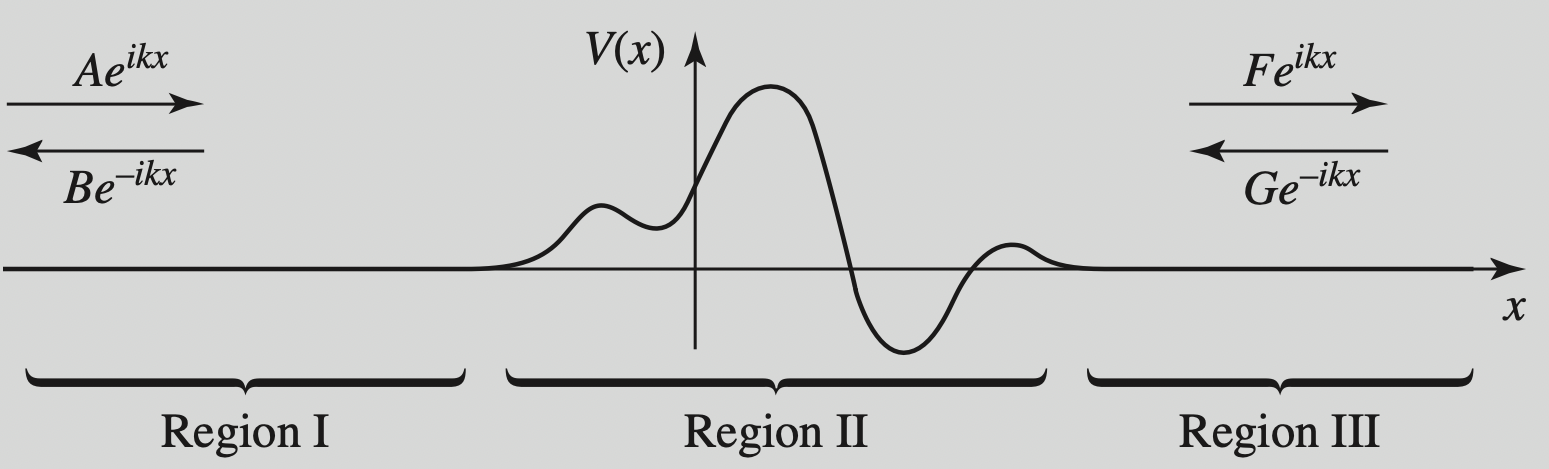
\includegraphics[width=1\linewidth]{./figures/arbitrary_V.png}
    \caption{Scattering from an arbitrary localized potential ($V(x)=0$ except for Region II)}
    \label{fig:arbitrary localized potential}
\end{wrapfigure}
\begin{align}
    T = \frac{1}{|M_{22}|^2}; \qquad R+T = 1
\end{align}
\subsection*{\underline{Spherical Coordinates:}}
$$
    \begin{aligned}
         & \hat{\mathbf{r}}=\sin \theta \cos \phi \hat{\mathbf{x}}+\sin \theta \sin \phi \hat{\mathbf{y}}+\cos \theta \hat{\mathbf{z}}          \\
         & \hat{\boldsymbol{\theta}}=\cos \theta \cos \phi \hat{\mathbf{x}}+\cos \theta \sin \phi \hat{\mathbf{y}}-\sin \theta \hat{\mathbf{z}} \\
         & \hat{\boldsymbol{\phi}}=-\sin \phi \hat{\mathbf{x}}+\cos \phi \hat{\mathbf{y}}
    \end{aligned}
$$
$$
    \begin{aligned}
         & \hat{\mathbf{x}}=\sin \theta \cos \phi \hat{\mathbf{r}}+\cos \theta \cos \phi \hat{\boldsymbol{\theta}}-\sin \phi \hat{\boldsymbol{\phi}} \\
         & \hat{\mathbf{y}}=\sin \theta \sin \phi \hat{\mathbf{r}}+\cos \theta \sin \phi \hat{\boldsymbol{\theta}}+\cos \phi \hat{\boldsymbol{\phi}} \\
         & \hat{\mathbf{z}}=\cos \theta \hat{\mathbf{r}}-\sin \theta \hat{\boldsymbol{\theta}}
    \end{aligned}
$$
\subsection*{\underline{Identical Particles:}}
Particles that share the same intrinsic properties: mass, charge, spin, magnetic moment, \dots etc. Identical particles are indistinguishable
\begin{equation}
    \Psi(1, 2, \dots, i, \dots, j, \dots, N)=\pm\Psi(1, 2, \dots, j, \dots, i, \dots, N)
\end{equation}
are either symmetric for Bosons (integer spin particles) or antisymmetric for Fermions (half integer spin particles) under exchange of any two particles.\\
$\implies$ Pauli Exclusion Principle: Two identical Fermions cannot occupy the same quantum state.
\begin{equation}
    \Psi_{Fermions}(R_1,R_2,\dots,R_N)= \frac{1}{\sqrt{N!}}
    \left(\begin{matrix}
            \Psi_1(R_1) & \Psi_2(R_1) & \dots  & \Psi_N(R_1) \\
            \Psi_1(R_2) & \Psi_2(R_2) & \dots  & \Psi_N(R_2) \\
            \vdots      & \vdots      & \vdots & \vdots      \\
            \Psi_1(R_N) & \Psi_2(R_N) & \dots  & \Psi_N(R_N)
        \end{matrix}\right)
\end{equation}
For Bosons use the same Slater-determinant by replacing all signs be + .
Spin $\frac{1}{2}$ particles can be in any of the following states:
\begin{enumerate}
    \item[] \underline{Singlet State (Antisymmetric state):} \begin{equation} \chi_s(s1,s2)=\frac{1}{\sqrt{2}}(\chi_{\uparrow}(s1)\chi_{\downarrow}(s2)-\chi_{\downarrow}(s1)\chi_{\uparrow}(s2)) \end{equation} with total spin s=0.
    \item[] \underline{Triplet States (Symmetric state):} with total spin $S_z=$1, 0, -1:
        \begin{gather}
            \chi_T(s_1, s_2) 
            \begin{cases}
                \chi_{1,1}(s_1,s_2)=\chi_{\uparrow}(s_1)\chi_{\uparrow}(s_2)       \\
                \chi_{-1,-1}(s_1,s_2)=\chi_{\downarrow}(s_1)\chi_{\downarrow}(s_2) \\
                \chi_{1,0}(s_1,s_2)=\frac{1}{\sqrt{2}}(\chi_{\uparrow}(s_1)\chi_{\downarrow}(s_2)+\chi_{\downarrow}(s_1)\chi_{\uparrow}(s_2))
            \end{cases}
        \end{gather}
\end{enumerate}
\subsection*{\underline{Electron Gas in Volume V:}}
Each eigenvalue in k-space occupy a volume $\frac{{(2\pi)^3}}{V}$ so that 2 for spin states:
\begin{equation} \sum_k f(k)=2\frac{V}{(2\pi)^3}\int d^3k f(k) \end{equation}
Highest occupied wave vector is called Fermi wave vector k$_F$
\begin{equation} k_F = (3\pi^2n)^{1/3}; \, n=\frac{N}{V} \,\, \text{Electronic Density}\end{equation}

\subsection*{\underline{Ground State of N Electrons in Volume V:}}

\begin{align}
     & E_F=\frac{\hbar^2k^2}{2m}
     & E=2\sum_k\frac{\hbar^2k^2}{2m}=\frac{3}{5}NE_F
     &                                                                                         \\
     & 2\frac{\Omega_k}{\frac{(2\pi)^3}{V}}=N=2\frac{\frac{4}{3}\pi k_F^3}{\frac{(2\pi)^3}{V}}
     & k_F = (3\pi^2n)^{1/3}
     &                                                                                         \\
     & n=\frac{N}{V}=\frac{1}{v}=\frac{1}{\frac{4}{3}\pi r_s^3}
     & r_s=\left(\frac{3}{4\pi n}\right)^{1/3}
     &                                                                                         \\
     & k_F = (3\pi^2n)^{1/3} = \frac{(9\pi /4)^{1/3}}{r_s}=\frac{1.92}{r_s}
\end{align}
\subsection*{\underline{Bloch Theorem in Solids:}}
\begin{gather}
    \psi (R+x)=e^{i k\cdot R} \psi (x)\\
    \text{\underline{In $3D$:}}\quad k_i = \frac{2\pi n_i}{L}; \quad i=x, y, z;\quad n=0, \pm1, \pm 2, ... \Rightarrow dn = \frac{V}{(2\pi)^3} dk^3\\
    \sum_{k\sigma}F(k, \sigma)= \frac{V}{(2\pi)^3} \sum_\sigma \int_{}  d k^3 F(k, \sigma)
\end{gather}
\subsection*{\underline{Probability Distributions:}}
\paragraph{}We have three distributions, one for classical particles (Maxwell-Boltzmann) and two for undistinguishable particles (Fermi-Dirac for fermions and Bose-Einstein for bosons). Their equations are the following:
\begin{gather}
    P(E)=\frac{1}{e^{\beta(E -E_f)}+1} \qquad \text{Fermi--Dirac Dist.}\\
    P(E)=\frac{1}{e^{\beta(E -\mu)}-1} \qquad \text{Bose--Einstein Dist.}\\
    P(E)=\frac{1}{e^{\beta(E -\mu)}} \qquad \text{Maxwell--Boltzmann Dist.}\\
    \text{Where $\beta=\frac{1}{k_B T}$}
\end{gather}
\paragraph{}The plots of these distributions for different temperatures:
\begin{center}
    \frame{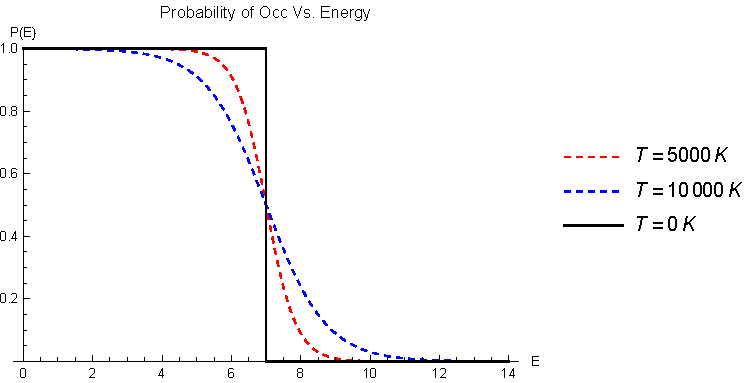
\includegraphics[width=13.5cm]{./figures/pt1.pdf}}\\
    \textbf{Figure 1:} Fermi--Dirac Dist. when $E_f=7eV$. For fermions\\
\end{center}
\par
\begin{center}
    \frame{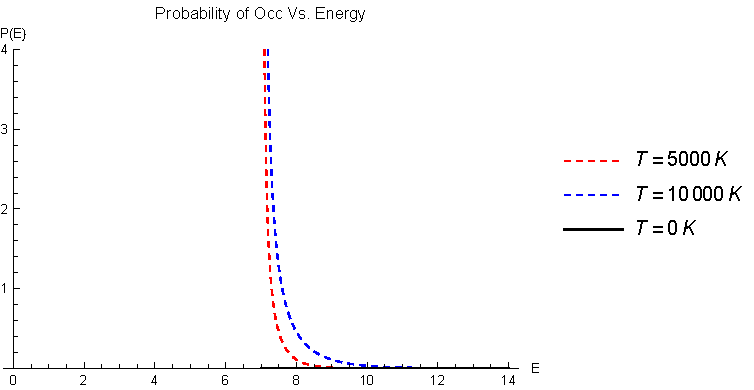
\includegraphics[width=13.5cm]{./figures/pt2.pdf}}\\
    \textbf{Figure 2:} Bose--Einstein Dist. when $\mu=7eV$. For bosons\\
\end{center}
\begin{center}
    \frame{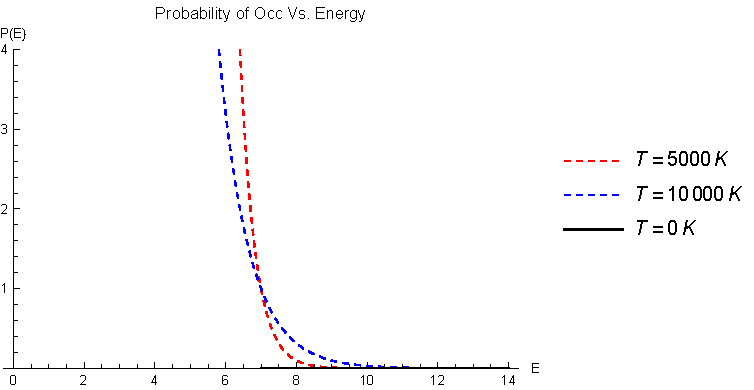
\includegraphics[width=13.5cm]{./figures/pt3.pdf}}\\
    \textbf{Figure 3:} Maxwell--Boltzmann Dist. when $\mu=7eV$. For bosons\\
\end{center}
\subsection*{\underline{Non-Degenerate Perturbation Theory}}
\begin{align}
     & H = H^0 + \lambda H' = H(\lambda)                                         \\
     & H(\lambda) \psi_n (\lambda) = E_n (\lambda) \psi_n (\lambda)              \\
     & \psi_n(\lambda) = \psi_n^0 + \lambda \psi_n^1 + \lambda^2 \psi_n^2+\cdots \\
     & E_n(\lambda) = E_n^0 + \lambda E_n^1 + \lambda^2 E_n^2 + \cdots           \\
     & \text{Assume }\psi_n(\lambda), \, E_n(\lambda) \text{ converges}          \\
\end{align}
\begin{align}
    \lambda^0: \quad & H^0|\psi_n^0\rangle = E_n^0 |\psi_n^0\rangle             \\
    \lambda^1: \quad & H^0|\psi_n^1\rangle + H'\psi_n^0 = E_n^0|\psi_n^1\rangle
    + E_n^1|\psi_n^0\rangle                                                     \\
    \lambda^2: \quad & H^0|\psi_n^2\rangle + H'\psi_n^1 = E_n^0|\psi_n^2\rangle
    + E_n^1|\psi_n^1\rangle + E_n^2|\psi_n^0\rangle
\end{align}
\begin{align}
    E_n^1            & = \langle\psi_n^0|H'|\psi_n^0\rangle                            \\
    |\psi_n^1\rangle & = \sum_{m\ne n} \frac{\langle \psi_m^0|H'|
    \psi_n^0\rangle}{E_n^0 - E_m^0} |\psi_m^0\rangle                                   \\
    E_n^2            & = \langle \psi_n^0 | H' | \psi_n^1\rangle                       \\
    E_n^2            & = \sum_{m\ne n} \frac{\left| \langle\psi_m^0|H'|\psi_n^0\rangle
        \right|^2}{E_n^0 - E_m^0}
\end{align}

Let $| \psi_1^0 \rangle$ and $| \psi_2^0 \rangle$ be degenerate states of $H^0$, then
\begin{align}
    H' = \begin{bmatrix}
        H'_{11} & H'_{12} \\
        H'_{21} & H'_{22} \\
    \end{bmatrix}; \quad \text{where} \quad
    H'_{ij} = \langle \psi_i^0 | H' | \psi_j^0 \rangle
\end{align}
\begin{align}
    | H' - E^1 I | = \begin{bmatrix}
        H'_{11} - E^1 & H'_{12} \\
        H'_{21} & H'_{22} - E^1 \\
    \end{bmatrix} \begin{bmatrix}
        \alpha_1 \\
        \alpha_2
    \end{bmatrix} = \begin{bmatrix}
        0 \\ 0
    \end{bmatrix}
\end{align}
\begin{align}
    E^1_\pm = \frac{1}{2}\, \left[ H'_{11} + H'_{22} \pm \sqrt{(H'_{11}-H'_{11})^2 + 4|H'_{12}|^2} \right]
    \quad \text{and} \quad |\psi_\pm \rangle = \alpha_1 |\psi_1^0 \rangle + \alpha_2 |\psi_2^0 \rangle
\end{align}

\end{document}